\documentclass[conference]{IEEEtran}
\IEEEoverridecommandlockouts
% The preceding line is only needed to identify funding in the first footnote. If that is unneeded, please comment it out.
\usepackage{cite}
\usepackage{amsmath,amssymb,amsfonts}
\usepackage{algorithmic}
\usepackage{graphicx}
\usepackage{textcomp}
\usepackage{xcolor}
\def\BibTeX{{\rm B\kern-.05em{\sc i\kern-.025em b}\kern-.08em
    T\kern-.1667em\lower.7ex\hbox{E}\kern-.125emX}}
\begin{document}

\title{Classification of Brain Tumors by Image Processing and Ensemble Learning\\}

\author{\IEEEauthorblockN{1\textsuperscript{st} Hakan Tekgul}
\IEEEauthorblockA{\textit{Electrical and Computer Engineering} \\
\textit{Georgia Institute of Technology}\\
Metz, France \\
htekgul3@gatech.edu}
\and
\IEEEauthorblockN{2\textsuperscript{nd} Jad Sinno}
\IEEEauthorblockA{\textit{Electrical and Computer Engineering} \\
\textit{Georgia Institute of Technology}\\
Metz, France \\
jsinno3@gatech.edu}
\and
\IEEEauthorblockN{3\textsuperscript{rd} Madhur Gupta}
\IEEEauthorblockA{\textit{Electrical and Computer Engineering} \\
\textit{Georgia Institute of Technology}\\
Metz, France \\
mgupta325@gatech.edu}
}

\maketitle

\begin{abstract}
When diagnosed at a late stage, brain cancers and tumors provide very short life expectancy and a high mortality rate because of their aggressive nature. In order to diagnose and detect the tumor on the brain at the earliest stage possible, various medical imaging techniques such as Computed Tomography (CT) or Magnetic Resonance Imaging (MRI) are used. Unfortunately, the diagnosis and treatment of the tumor depends highly on the physician’s medical knowledge. Hence, many different systems have been proposed in the past decade to automatically detect brain tumors by using machine learning. One major problem with these approaches is the fact that they usually need lots of training data (MRI Scans).  

In this project, we detect brain tumors from MRI images with a limited amount of training data, around 120 images. Specifically, we use an ensemble learning approach that is based on Support Vector Machines (SVM). After applying image processing techniques such as low-pass filtering to all the images, the most common prediction from different SVM classifiers is chosen for a testing image. Validation accuracies are used to select the best image processing techniques and their optimal parameters. Our experimental results suggest that the Ensemble Classifier achieves an accuracy of 87\% with low time complexity.
\end{abstract}

\begin{IEEEkeywords}
Brain Tumor, Image Classification, Ensemble Learning, Medical Imaging, SVM
\end{IEEEkeywords}

\section{Introduction}\label{intro}
\subsection{Motivation}
% Explain the motivation behind project and goal of project
Brain cancers and tumors affect the life of humans negatively, as abnormal growth of brain cells damage the functioning of the brain and might even lead to death. With increased usage of cell phones, the incidence rate of brain tumors is predicted to rise rapidly \cite{b1}. Furthermore, the mortality rate of brain cancers have also been increasing constantly in the past decade \cite{b2}. In order to reduce the mortality rate and treat brain tumors, diagnosis should be done in the earliest stage possible. 

Medical imaging is used to diagnose and visualize different types of tumors in the human body. Various medical imaging techniques such as CT Scan, MRI, or X-Ray is used in hospitals for diagnosis. Magnetic Resonance Imaging (MRI) is generally used for brain tumor diagnosis as it shows the inside of the brain with contrast \cite{b7}. With the use of MRI, brain tumors are identified as soon as possible by many physicians. However, some MRI scans are hard to read and there is a chance that physicians can make a mistake during diagnosis. When a physician decides that a tumor in the brain does not exist but in reality there is a tumor, a false negative diagnosis occurs and such diagnosis can be catastrophic for the patient. Hence, many different systems have been proposed in the past decade that automatically identifies brain tumors in an MRI scan. Even though most of these approaches have good accuracy and results, they usually need a huge number of training data and computation resources. Therefore, new approaches for brain tumor classification must be considered. 

In this work, we propose to detect brain tumors from MRI images with a limited amount of training data. Specifically, we use image processing and ensemble learning through Support Vector Machines (SVM) to classify whether an MRI scan has a tumor or not. Our main goal in this study is to maximize the classification accuracy and minimize the number of false negatives. We use different image processing techniques, inluding Low-Pass Filter (LPF), High-Pass Filter (HPF), Median Filter (MF), and Low-Pass - High-Pass Filter (LPF+HPF). Then, we apply different machine learning algorithms such as k-NN, SVM, and Neural Networks (NN). To summarize, we make three main contributions in this paper:
\begin{itemize}
  \item We apply different image filters to MRI scans and analyze the best processing technique for tumor detection.
  \item We experiment with three different machine learning algorithms and state their accuracy for differrent image processing techniques.
  \item We propose an ensemble learning approach that successfully identifies a tumor in the brain with a minimum number of false negatives. 
\end{itemize}
Our experimental results suggest that LPF+HPF is the best filter to use for tumor detection, with an average classification accuracy of 84\%. Additionaly, we observed that Support Vector Machines (SVM) gives the optimal results in terms of classification. Finally, our ensemble learning approach that is based on different filters and Support Vector Machines outputs a classification accuracy of 87\% and a 2\% false negative rate. 

\subsection{Related Work} 
% Discuss some related work. Provide around 5-6 projects about tumor classification and summarize their improvements/results
% DO NOT FORGET TO CITE
The development of brain tumor recoginition has been increasing in the past decade. Many appraoches have been proposed that build different models for MRI scan classification. Some approaches use image processing techniques, whereas some approaches are solely focused on deep learning to identify tumors. Some of the related work to our project is presented below. 

Firstly, Praveen \cite{b3} introduced the use of image processing and segmentation for the problem of tumor detection. Different imaging filters such as median filter, wiener filter are used to process images and different edge detection and feature extraction techniques are used for classification. Then, Gaikwad et. al \cite{b4} experimented with dimensionality reduction of MRI images using Principal Component Analysis (PCA) and developed a Probabilistic Neural Network for tumor classification. 

Apart from image processing or segmentation, Ari et. al \cite{b5} used deep learning to classify brain tumors by focusing on extreme learning machine local receptive fields (ELM-LRF) based tumor classification. Their work showed very promising accuracy results. Similarly, Seetha et. al \cite{b6} used convolutional neural networks with deep architecture and small kernels to classify brain tumors. By setting the weights of neurons to small values, their results were also very promising. The only problem with deep learning approaches is the fact that they usually need lots of training data. 

As compared to these works, we experiments with a wide range of image processing techniques and we analyze the best imaging filter to use for tumor detection. Even though our accuracy value is not very high compared to works that used deep learning, we propose a classifier that can work well with limited amount of training data. To the best of our knowledge, this project is the first to apply ensemble learning for tumor identification. Finally, this work is also the only one that tries to minimize false negatives as well as accuracy, and discuss the results. Hence, we believe our contribution to brain tumor classification is significant.


\section{Methodology}\label{method}
% Put the flowchart here 
\begin{figure}[h]
\centering
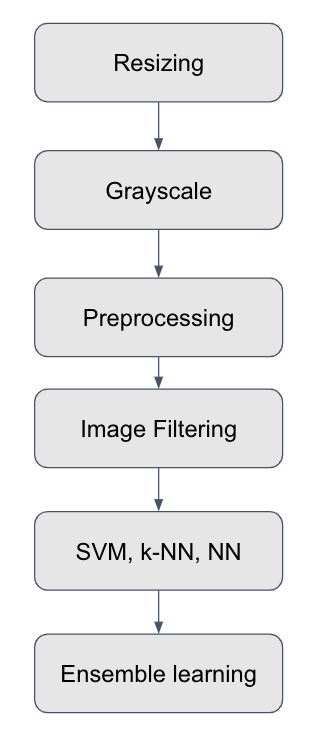
\includegraphics[scale=0.4]{flowchart}
\caption{Flowchart of the project that summarizes our process for our experiments.}
\end{figure}
% Explain our methodology behind the project
% Talk briefly about resizing and grayscale. Maybe put the graph on image sizes? 

For this project, we used an MRI Scan dataset that has a total of 255 images. The dataset is balanced, where there are 156 positive images and 99 negative images. From the 255 images, 70\% is used for training and 30\% is used for testing. After that, all the images are resized to a certain size through bicubic interpolation and each image is converted to grayscale. This was because the MRI scans usually consist of black and white pixels and RGB colors does not contribute to identification of tumors. Note that the methodology behind this project is shown in Figure 1.

\subsection{Image Preprocessing}
% Describe the equalization and contrast images
% Add histograms, equalized and contrast image examples, visualize sigmoid etc. 
To be fed into the classifier, the images had to be resized to a common size. In our case, we resized them all to $350\times300\: px$ around which most images were distributed (Figure 2). The method used is either downsampling for downscaling or upsampling the images using bicubic interpolation for upscaling.
\begin{figure}[h]
\centering
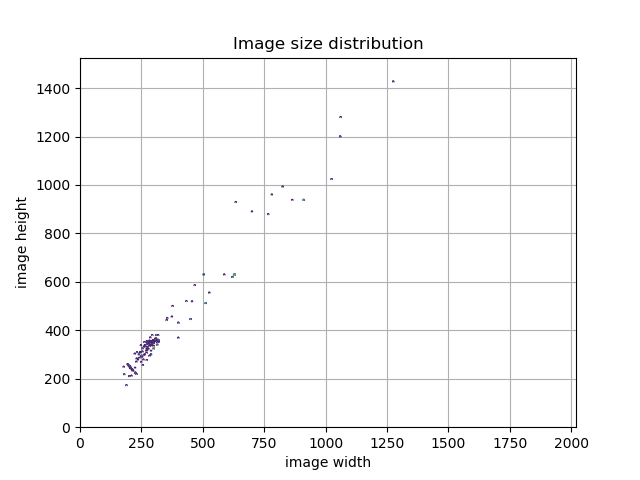
\includegraphics[scale=0.5]{figures/Image_size_distribution.png}
\caption{Original image size distribution in pixels.}
\end{figure}

From this homogeneous dataset, two sub-datasets were created : the first one adds contrast to the images, the second one equalizes the histograms.\\
\paragraph*{Contrast addition}
In the following example (Figure 3), the tumor stands out by the luminance difference with healthy brain tissue. Thus our hypothesis is that adding contrast can help emphasizing the even more the tumor. The method used is a sigmoïd transformation : for every pixel $x \in [0;255]$, $$x\leftarrow x\times \frac{1}{1+e^{-0.02(x-127)}}$$
\begin{figure}[h]
\centering
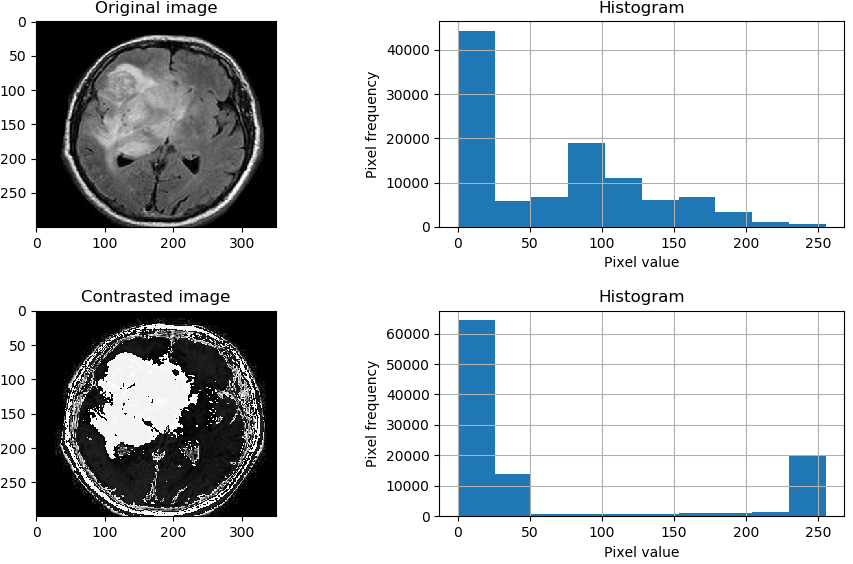
\includegraphics[scale=0.33]{figures/Contrasting.png}
\caption{Sample image of a brain having tumor and associated histogram before and after adding contrast.}
\end{figure}

\paragraph*{Equalization}
In the following example (Figure 4), there is no clear tumor (and in fact there is no tumor, but we don't know it beforehand), and most pixels are concentrated around a certain gray value, making it difficult to distinguish details. Thus our hypothesis is that histogram equalization can help distinguishing details, for example distinguishing a tumor when its luminance is close to healthy brain tissue.
\begin{figure}[h]
\centering
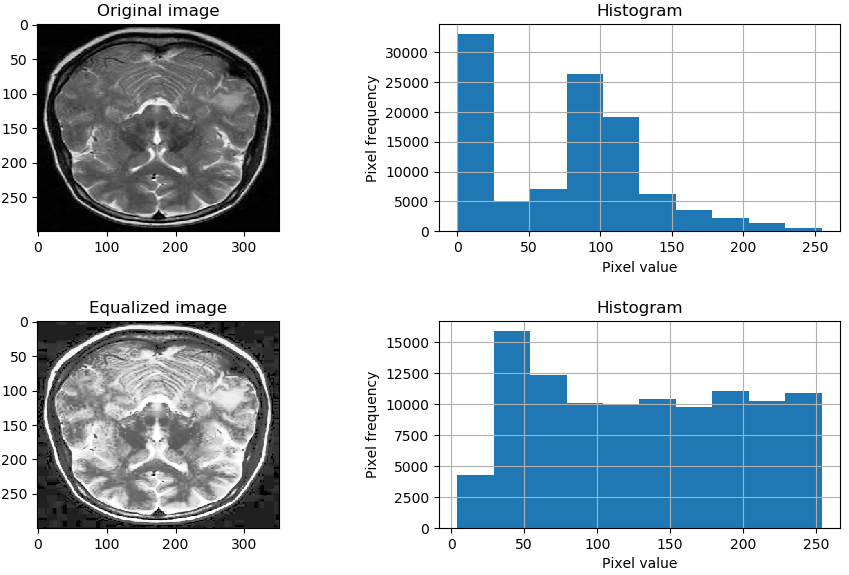
\includegraphics[scale=0.33]{figures/Equalizing.png}
\caption{Sample image of a brain without tumor and associated histogram before and after equalizing histograms.}
\end{figure}

\subsection{Image Filtering}
% Describe and explain the different filters 
A low pass filter is used for smoothing the images and it also helps in removing the high frequency components and noise in the image. We have applied this filter with various sigma values to the contrast and equalized images.
We have also used the high pass filter with various sigma values on the contrast and equalized images. It helps us to do the training of dataset and classification on the tumor region in the image using the high frequency content in the image.
We have also combined the above two filters to filter the images in our dataset. So, we first applied the low pass filter and then the high pass filter and it helped us to remove the noise in the images and then perform the classification on the relatively high frequency content in the image.
Finally we have used the median filter to filter the images as it gives good quality images for the classification part of our project. It takes the median of the neighborhood of each of the pixels in the image and replaces the specified pixel by that value. 
% Provide examples of filtered images (one image from each filtering is fine)
\begin{figure}[h]
\centering
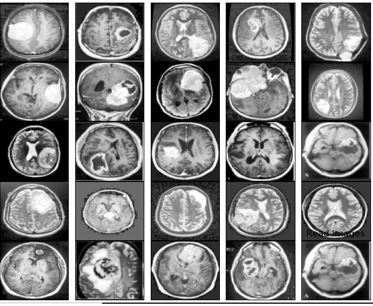
\includegraphics[scale=0.43]{figures/lpf.JPG}
\caption{Low pass filtered images.}
\end{figure}
\begin{figure}[h]
\centering
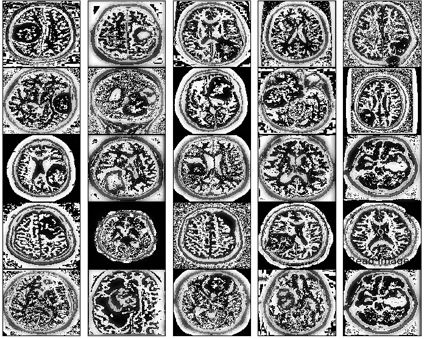
\includegraphics[scale=0.40]{figures/hpf.JPG}
\caption{High pass filtered images.}
\end{figure}
\begin{figure}[h]
\centering
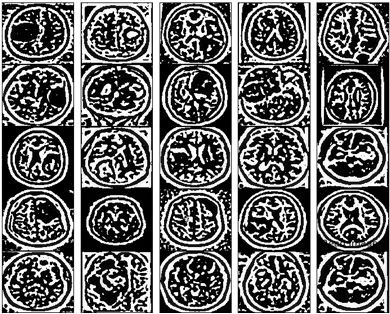
\includegraphics[scale=0.43]{figures/lpf_hpf.JPG}
\caption{Low pass + high pass filtered images.}
\end{figure}
\begin{figure}[h]
\centering
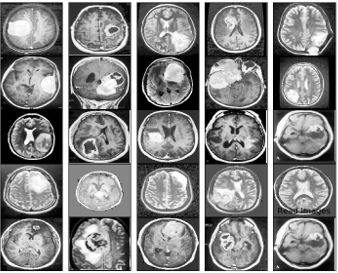
\includegraphics[scale=0.43]{figures/median.JPG}
\caption{Median filtered images.}
\end{figure}

% Note that, the filters used are GAUSSIAN --> would be nice to visualize the filters in a graph
\begin{figure}[h]
\centering
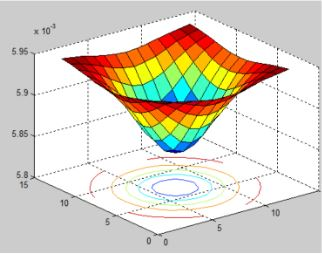
\includegraphics[scale=0.4]{figures/hpf_filter.JPG}
\caption{Visualization of HPF.}
\end{figure}
\begin{figure}[h]
\centering
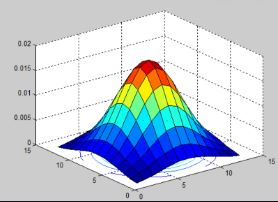
\includegraphics[scale=0.4]{figures/lpf_filter.JPG}
\caption{Visualization of LPF.}
\end{figure}

\subsection{Machine Learning}
% Briefly describe the machine learning algorithms 
After creating the contrasted, equalized versions of the dataset and applying different image filters, classification experiments are conducted by applying three different machine learning algorithms. As stated before, k-Nearest Neighbors (kNN), Support Vector Machines (SVM), and Artificial Neural Networks (NN) are applied on our data. k-NN is chosen because of its simplicity and the fact that our images are not that complex in nature. SVM, on the other hand, is selected as a machine learning algorithm because it can work very well with low amount of training data and it handles outliers very well. Finally, because image classification is usually done with Neural Networks, we chose NN as the last algorithm. 

% Cross validation
After choosing the algorithms, the dataset is split into training, validation, and testing. As stated before, 70\% of data is used for training and 30\% of training set is used for validation. Then, all the specified machine learning algorithms are applied to the training set and cross-validation approach is used to tune the parameters of each algorithm. After the optimization of the classifiers, accuracy results are collected for different classifiers, different image filters, and their different sigma values. Such results are presented in section 3. 

% Ensemble Learning
Finally, best 8 classifier/filter/sigma combinations that had the maximum but different accuracies are selected for ensemble learning. Ensemble learning is applied because some of the classifiers had overfitting and there was a need to generalize the data better. At the end, the most common prediction from the 8 classifiers is taken as the final result. In the case of a tie, the classifier predicts a positive instance to lower the number of false negatives.

\section{Experimental Results}\label{results}
% Provide experimental results here
% Provide 3 different tables --> cluster all k-NN results together into one table, same for SVM and NN
% Learning curves, validation curves
% Final Confusion Matrix 

\section{Analysis of Results}\label{analysis}
% Detailed analysis of all results and process
% Analyze the results for each filter, different sigma values, and for each ML algorithm
% Which image filter worked the best? --> LPF+HPF analyze other ones too
% Which ML algorithm worked the best? --> SVM analyze other ones too --> why did NN not do good? 
% How helpful was ensemble learning? Why --> generalization
% Discuss false negatives and accuracy 

\section{Conclusion and Future Work}\label{conclusion}
% Briefly summarize main ideas of project
% Discuss future work such as tumor segmentation


\begin{thebibliography}{00}
\bibitem{b1} Hallberg Ö, Morgan LL (2011) The Potential Impact of Mobile Phone Use on Trends in Brain and CNS Tumors. J Neurol Neurophysiol S5. doi:10.4172/2155-9562.S5-003
\bibitem{b2} Australian Institute of Health and Welfare 2019. Cancer in Australia 2019. Cancer series no.119. Cat. no. CAN 122. Canberra: AIHW.
\bibitem{b3} Gamage, Praveen. (2017). Identification of Brain Tumor using Image Processing Techniques. 
\bibitem{b4} Gaikwad, Sonali \& Joshi, M.. (2015). Brain Tumor Classification using Principal Component Analysis and Probabilistic Neural Network. International Journal of Computer Applications. 120. 5-9. 10.5120/21205-3885.
\bibitem{b5} Ari, Ali \& Hanbay, Davut. (2018). Deep learning based brain tumor classification and detection system. TURKISH JOURNAL OF ELECTRICAL ENGINEERING \& COMPUTER SCIENCES. 26. 2275-2286. 10.3906/elk-1801-8.
\bibitem{b6} Seetha, J. \& Raja, S.. (2018). Brain Tumor Classification Using Convolutional Neural Networks. Biomedical and Pharmacology Journal. 11. 1457-1461. 10.13005/bpj/1511. 
\bibitem{b7} Kernick DP, Ahmed F, Bahra A, et al. Imaging patients with suspected brain tumour: guidance for primary care. Br J Gen Pract. 2008;58(557):880–885. doi:10.3399/bjgp08X376203.
\end{thebibliography}

\end{document}
